\renewcommand{\FiscalYear}{(fiscal year 2024--2025)}
% Economic Impact Analysis Report
% Generated: 2025-10-16 10:30:27
% Conservative Budget Estimation Analysis

\section{Economic Impact Analysis}
\label{sec:economic_impact}

This section presents the economic impact analysis for each budget allocation model. The conservative budget estimate is defined as the maximum of the actual cost and predicted cost for each case: $\text{Conservative} = \max(\text{Actual}, \text{Predicted})$. This approach ensures adequate funding while accounting for model uncertainty.

\subsection{Model 1: Impact Analysis}
\label{subsec:model1_impact}

\begin{table}[htbp]
\centering
\small
\caption{Model 1: Economic Impact Summary \FiscalYear}
\label{tab:model1_impact_summary}
\begin{tabular}{lrr}
\toprule
\textbf{Metric} & \textbf{Value} & \textbf{Per Client} \\
\midrule
Sample Size & 35,444 & --- \\
\midrule
Total Actual Cost & \$1,680,682,853.91 & \$47,417.98 \\
Total Predicted Cost & \$1,322,238,048.82 & \$37,304.99 \\
Total Conservative Budget & \$1,908,875,018.24 & \$53,856.08 \\
\midrule
\textbf{Economic Impact} & \textbf{\$+228,192,164.33} & \textbf{\$+6,438.10} \\
Impact Percentage & 13.58\% & --- \\
\midrule
Cases Over Budget & 17,173 & 48.5\% \\
\midrule
Model $R^2$ (Test) & 0.4300 & --- \\
RMSE (Test) & \$33,718.68 & --- \\
\bottomrule
\end{tabular}
\end{table}

\begin{table}[htbp]
\centering
\small
\caption{Model 1: Economic Impact by Budget Quartile \FiscalYear}
\label{tab:model1_impact_quartile}
\begin{tabular}{lrrrrr}
\toprule
\textbf{Budget Quartile} & \textbf{N} & \textbf{Mean Actual} & \textbf{Mean Conservative} & \textbf{Impact} & \textbf{Impact \%} \\
\midrule
Q1 (Low) & 8,861 & \$1,815.61 & \$14,048.92 & \$+108,399,342.29 & +971.31\% \\
Q2 & 8,861 & \$16,963.90 & \$22,703.76 & \$+50,860,912.56 & +51.47\% \\
Q3 & 8,861 & \$57,199.58 & \$62,808.44 & \$+49,700,093.71 & +10.28\% \\
Q4 (High) & 8,861 & \$113,692.83 & \$115,863.22 & \$+19,231,815.77 & +2.47\% \\
\bottomrule
\end{tabular}
\end{table}

\begin{table}[htbp]
\centering
\small
\caption{Model 1: Distribution by Impact Level \FiscalYear}
\label{tab:model1_impact_distribution}
\begin{tabular}{lrrrrr}
\toprule
\textbf{Impact Level} & \textbf{N} & \textbf{\%} & \textbf{Mean Actual} & \textbf{Mean Impact} & \textbf{Impact \%} \\
\midrule
No Change & 18,271 & 51.5\% & \$71,551.35 & \$+0.00 & +0.00\% \\
Small Increase (0-10\%) & 1,785 & 5.0\% & \$60,779.33 & \$+2,895.91 & +4.86\% \\
Moderate Increase (10-25\%) & 1,988 & 5.6\% & \$54,121.24 & \$+9,096.24 & +17.07\% \\
Large Increase (>25\%) & 13,400 & 37.8\% & \$11,737.62 & \$+15,294.00 & +681.58\% \\
\bottomrule
\end{tabular}
\end{table}

Tables~\ref{tab:model1_impact_summary} through \ref{tab:model1_impact_distribution} present detailed subgroup analyses, revealing how economic impact varies across age groups, living settings, budget levels, and impact categories. These breakdowns help identify which populations are most affected by prediction errors and where conservative budgeting has the greatest effect.

Figure~\ref{fig:model1_impact_histograms} presents the distribution analysis for Model 1, showing the distributions of actual costs, predicted costs, prediction errors, and conservative budget estimates.

\begin{figure}[htbp]
\centering
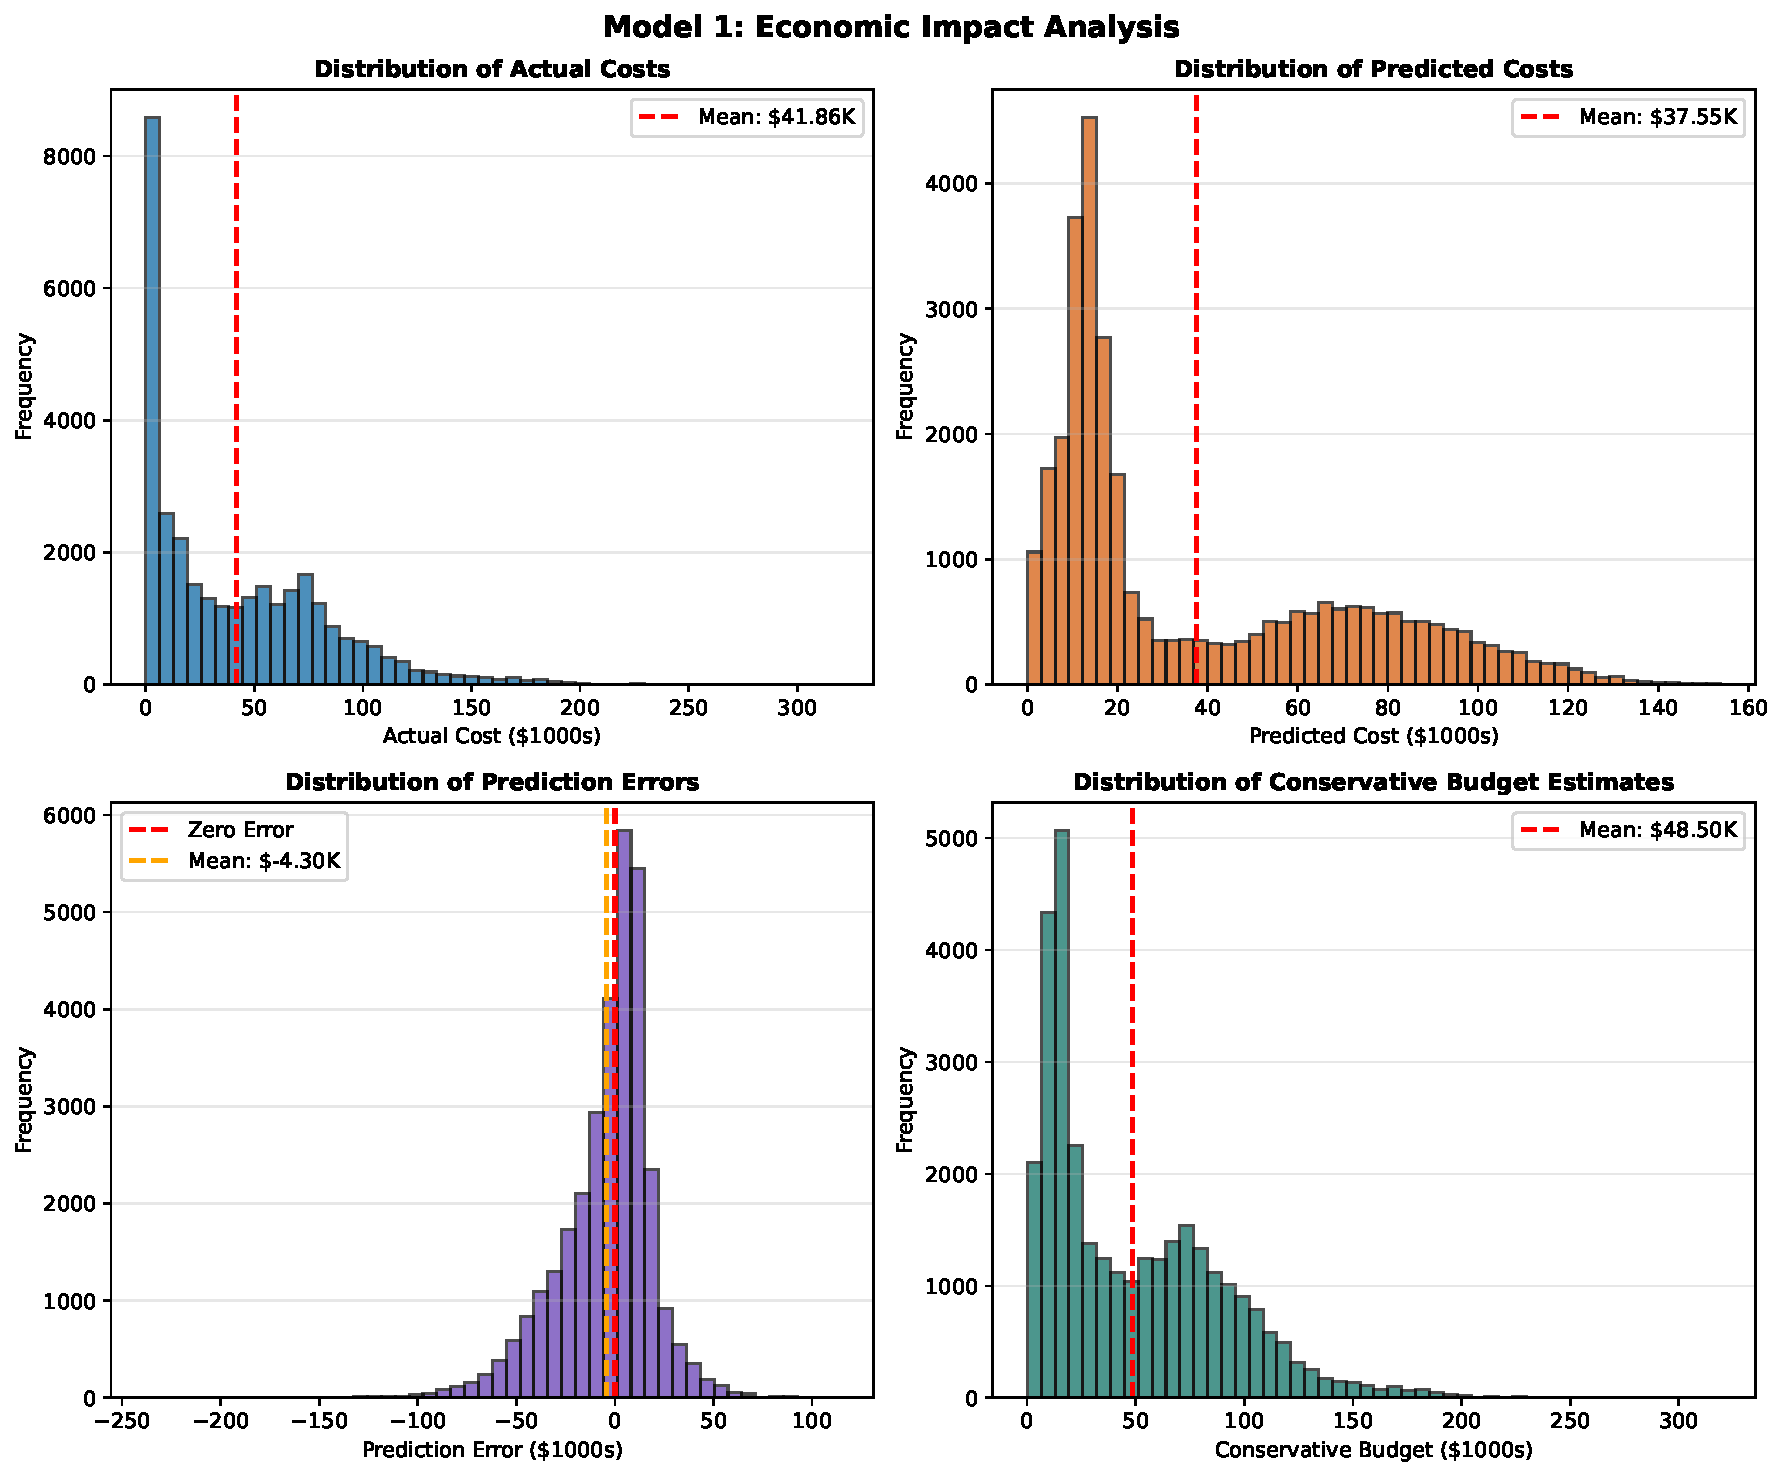
\includegraphics[width=0.95\textwidth]{figures/model_1_Impact_Histograms.pdf}
\caption{Model 1: Distribution of costs, predictions, errors, and conservative budget estimates. The conservative estimate takes the maximum of actual and predicted costs to ensure adequate funding \FiscalYear.}
\label{fig:model1_impact_histograms}
\end{figure}

The conservative budgeting approach for Model 1 would require an additional \$228,192,164.33 (13.58\%) compared to actual costs, averaging \$6,438.10 per client. The model under-predicted costs in 48.5\% of cases, necessitating the conservative approach to avoid budget shortfalls. Notably, 37.8\% of cases (13,400 clients) require large budget increases exceeding 25\%, highlighting the importance of the conservative approach for high-risk cases. 

\clearpage

\subsection{Model 2: Impact Analysis}
\label{subsec:model2_impact}

\begin{table}[htbp]
\centering
\small
\caption{Model 2: Economic Impact Summary \FiscalYear}
\label{tab:model2_impact_summary}
\begin{tabular}{lrr}
\toprule
\textbf{Metric} & \textbf{Value} & \textbf{Per Client} \\
\midrule
Sample Size & 35,444 & --- \\
\midrule
Total Actual Cost & \$1,680,682,853.91 & \$47,417.98 \\
Total Predicted Cost & \$1,612,314,909.62 & \$45,489.08 \\
Total Conservative Budget & \$2,078,656,644.10 & \$58,646.22 \\
\midrule
\textbf{Economic Impact} & \textbf{\$+397,973,790.19} & \textbf{\$+11,228.24} \\
Impact Percentage & 23.68\% & --- \\
\midrule
Cases Over Budget & 20,782 & 58.6\% \\
\midrule
Model $R^2$ (Test) & 0.4386 & --- \\
RMSE (Test) & \$33,463.23 & --- \\
\bottomrule
\end{tabular}
\end{table}

\begin{table}[htbp]
\centering
\small
\caption{Model 2: Economic Impact by Budget Quartile \FiscalYear}
\label{tab:model2_impact_quartile}
\begin{tabular}{lrrrrr}
\toprule
\textbf{Budget Quartile} & \textbf{N} & \textbf{Mean Actual} & \textbf{Mean Conservative} & \textbf{Impact} & \textbf{Impact \%} \\
\midrule
Q1 (Low) & 8,861 & \$1,815.61 & \$22,145.22 & \$+180,140,635.74 & +1,557.13\% \\
Q2 & 8,861 & \$16,963.90 & \$26,428.21 & \$+83,863,235.56 & +89.60\% \\
Q3 & 8,861 & \$57,199.58 & \$65,389.01 & \$+72,566,549.75 & +14.44\% \\
Q4 (High) & 8,861 & \$113,692.83 & \$120,622.45 & \$+61,403,369.14 & +7.38\% \\
\bottomrule
\end{tabular}
\end{table}

\begin{table}[htbp]
\centering
\small
\caption{Model 2: Distribution by Impact Level \FiscalYear}
\label{tab:model2_impact_distribution}
\begin{tabular}{lrrrrr}
\toprule
\textbf{Impact Level} & \textbf{N} & \textbf{\%} & \textbf{Mean Actual} & \textbf{Mean Impact} & \textbf{Impact \%} \\
\midrule
No Change & 14,662 & 41.4\% & \$77,734.19 & \$+0.00 & +0.00\% \\
Small Increase (0-10\%) & 1,862 & 5.3\% & \$64,148.83 & \$+3,108.52 & +4.85\% \\
Moderate Increase (10-25\%) & 2,252 & 6.4\% & \$60,998.59 & \$+10,518.38 & +17.26\% \\
Large Increase (>25\%) & 16,668 & 47.0\% & \$17,046.45 & \$+22,108.13 & +884.16\% \\
\bottomrule
\end{tabular}
\end{table}

Tables~\ref{tab:model2_impact_summary} through \ref{tab:model2_impact_distribution} present detailed subgroup analyses, revealing how economic impact varies across age groups, living settings, budget levels, and impact categories. These breakdowns help identify which populations are most affected by prediction errors and where conservative budgeting has the greatest effect.

Figure~\ref{fig:model2_impact_histograms} presents the distribution analysis for Model 2, showing the distributions of actual costs, predicted costs, prediction errors, and conservative budget estimates.

\begin{figure}[htbp]
\centering
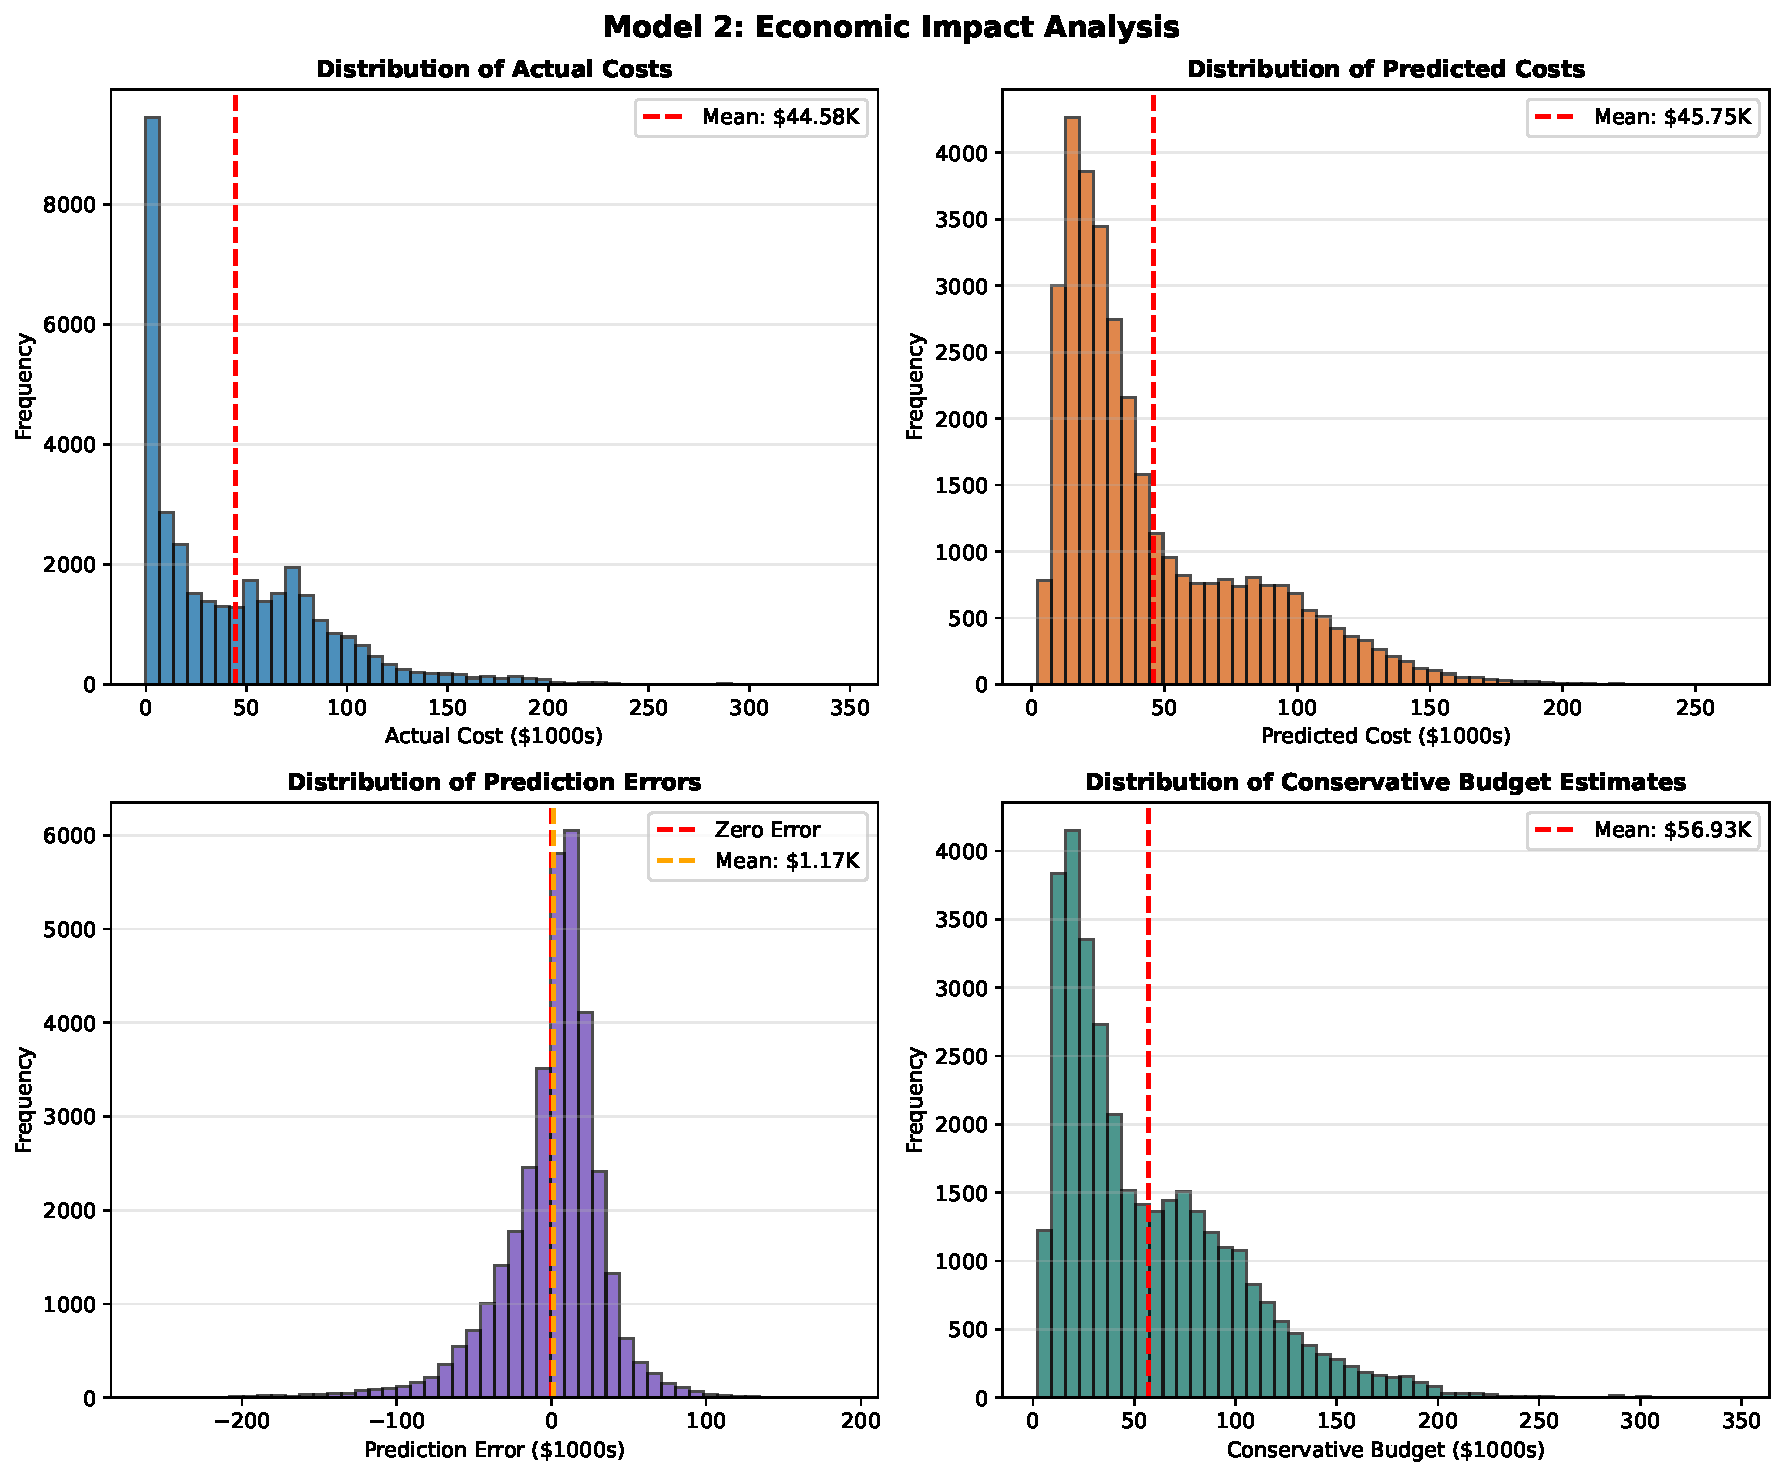
\includegraphics[width=0.95\textwidth]{figures/model_2_Impact_Histograms.pdf}
\caption{Model 2: Distribution of costs, predictions, errors, and conservative budget estimates. The conservative estimate takes the maximum of actual and predicted costs to ensure adequate funding \FiscalYear.}
\label{fig:model2_impact_histograms}
\end{figure}

The conservative budgeting approach for Model 2 would require an additional \$397,973,790.19 (23.68\%) compared to actual costs, averaging \$11,228.24 per client. The model under-predicted costs in 58.6\% of cases, necessitating the conservative approach to avoid budget shortfalls. Notably, 47.0\% of cases (16,668 clients) require large budget increases exceeding 25\%, highlighting the importance of the conservative approach for high-risk cases. 

\clearpage

\subsection{Model 3: Impact Analysis}
\label{subsec:model3_impact}

\begin{table}[htbp]
\centering
\small
\caption{Model 3: Economic Impact Summary \FiscalYear}
\label{tab:model3_impact_summary}
\begin{tabular}{lrr}
\toprule
\textbf{Metric} & \textbf{Value} & \textbf{Per Client} \\
\midrule
Sample Size & 35,444 & --- \\
\midrule
Total Actual Cost & \$1,680,682,853.91 & \$47,417.98 \\
Total Predicted Cost & \$1,397,240,560.07 & \$39,421.07 \\
Total Conservative Budget & \$1,950,387,953.94 & \$55,027.31 \\
\midrule
\textbf{Economic Impact} & \textbf{\$+269,705,100.03} & \textbf{\$+7,609.33} \\
Impact Percentage & 16.05\% & --- \\
\midrule
Cases Over Budget & 17,573 & 49.6\% \\
\midrule
Model $R^2$ (Test) & 0.4534 & --- \\
RMSE (Test) & \$33,018.58 & --- \\
\bottomrule
\end{tabular}
\end{table}

\begin{table}[htbp]
\centering
\small
\caption{Model 3: Economic Impact by Budget Quartile \FiscalYear}
\label{tab:model3_impact_quartile}
\begin{tabular}{lrrrrr}
\toprule
\textbf{Budget Quartile} & \textbf{N} & \textbf{Mean Actual} & \textbf{Mean Conservative} & \textbf{Impact} & \textbf{Impact \%} \\
\midrule
Q1 (Low) & 8,861 & \$1,815.61 & \$18,047.41 & \$+143,829,956.85 & +1,269.96\% \\
Q2 & 8,861 & \$16,963.90 & \$24,701.80 & \$+68,565,518.29 & +72.13\% \\
Q3 & 8,861 & \$57,199.58 & \$62,495.16 & \$+46,924,112.97 & +9.79\% \\
Q4 (High) & 8,861 & \$113,692.83 & \$114,864.88 & \$+10,385,511.91 & +1.39\% \\
\bottomrule
\end{tabular}
\end{table}

\begin{table}[htbp]
\centering
\small
\caption{Model 3: Distribution by Impact Level \FiscalYear}
\label{tab:model3_impact_distribution}
\begin{tabular}{lrrrrr}
\toprule
\textbf{Impact Level} & \textbf{N} & \textbf{\%} & \textbf{Mean Actual} & \textbf{Mean Impact} & \textbf{Impact \%} \\
\midrule
No Change & 17,871 & 50.4\% & \$73,432.24 & \$+0.00 & +0.00\% \\
Small Increase (0-10\%) & 1,854 & 5.2\% & \$60,511.84 & \$+2,818.21 & +4.76\% \\
Moderate Increase (10-25\%) & 2,014 & 5.7\% & \$51,734.09 & \$+8,593.00 & +16.80\% \\
Large Increase (>25\%) & 13,705 & 38.7\% & \$11,090.40 & \$+18,035.30 & +871.85\% \\
\bottomrule
\end{tabular}
\end{table}

Tables~\ref{tab:model3_impact_summary} through \ref{tab:model3_impact_distribution} present detailed subgroup analyses, revealing how economic impact varies across age groups, living settings, budget levels, and impact categories. These breakdowns help identify which populations are most affected by prediction errors and where conservative budgeting has the greatest effect.

Figure~\ref{fig:model3_impact_histograms} presents the distribution analysis for Model 3, showing the distributions of actual costs, predicted costs, prediction errors, and conservative budget estimates.

\begin{figure}[htbp]
\centering
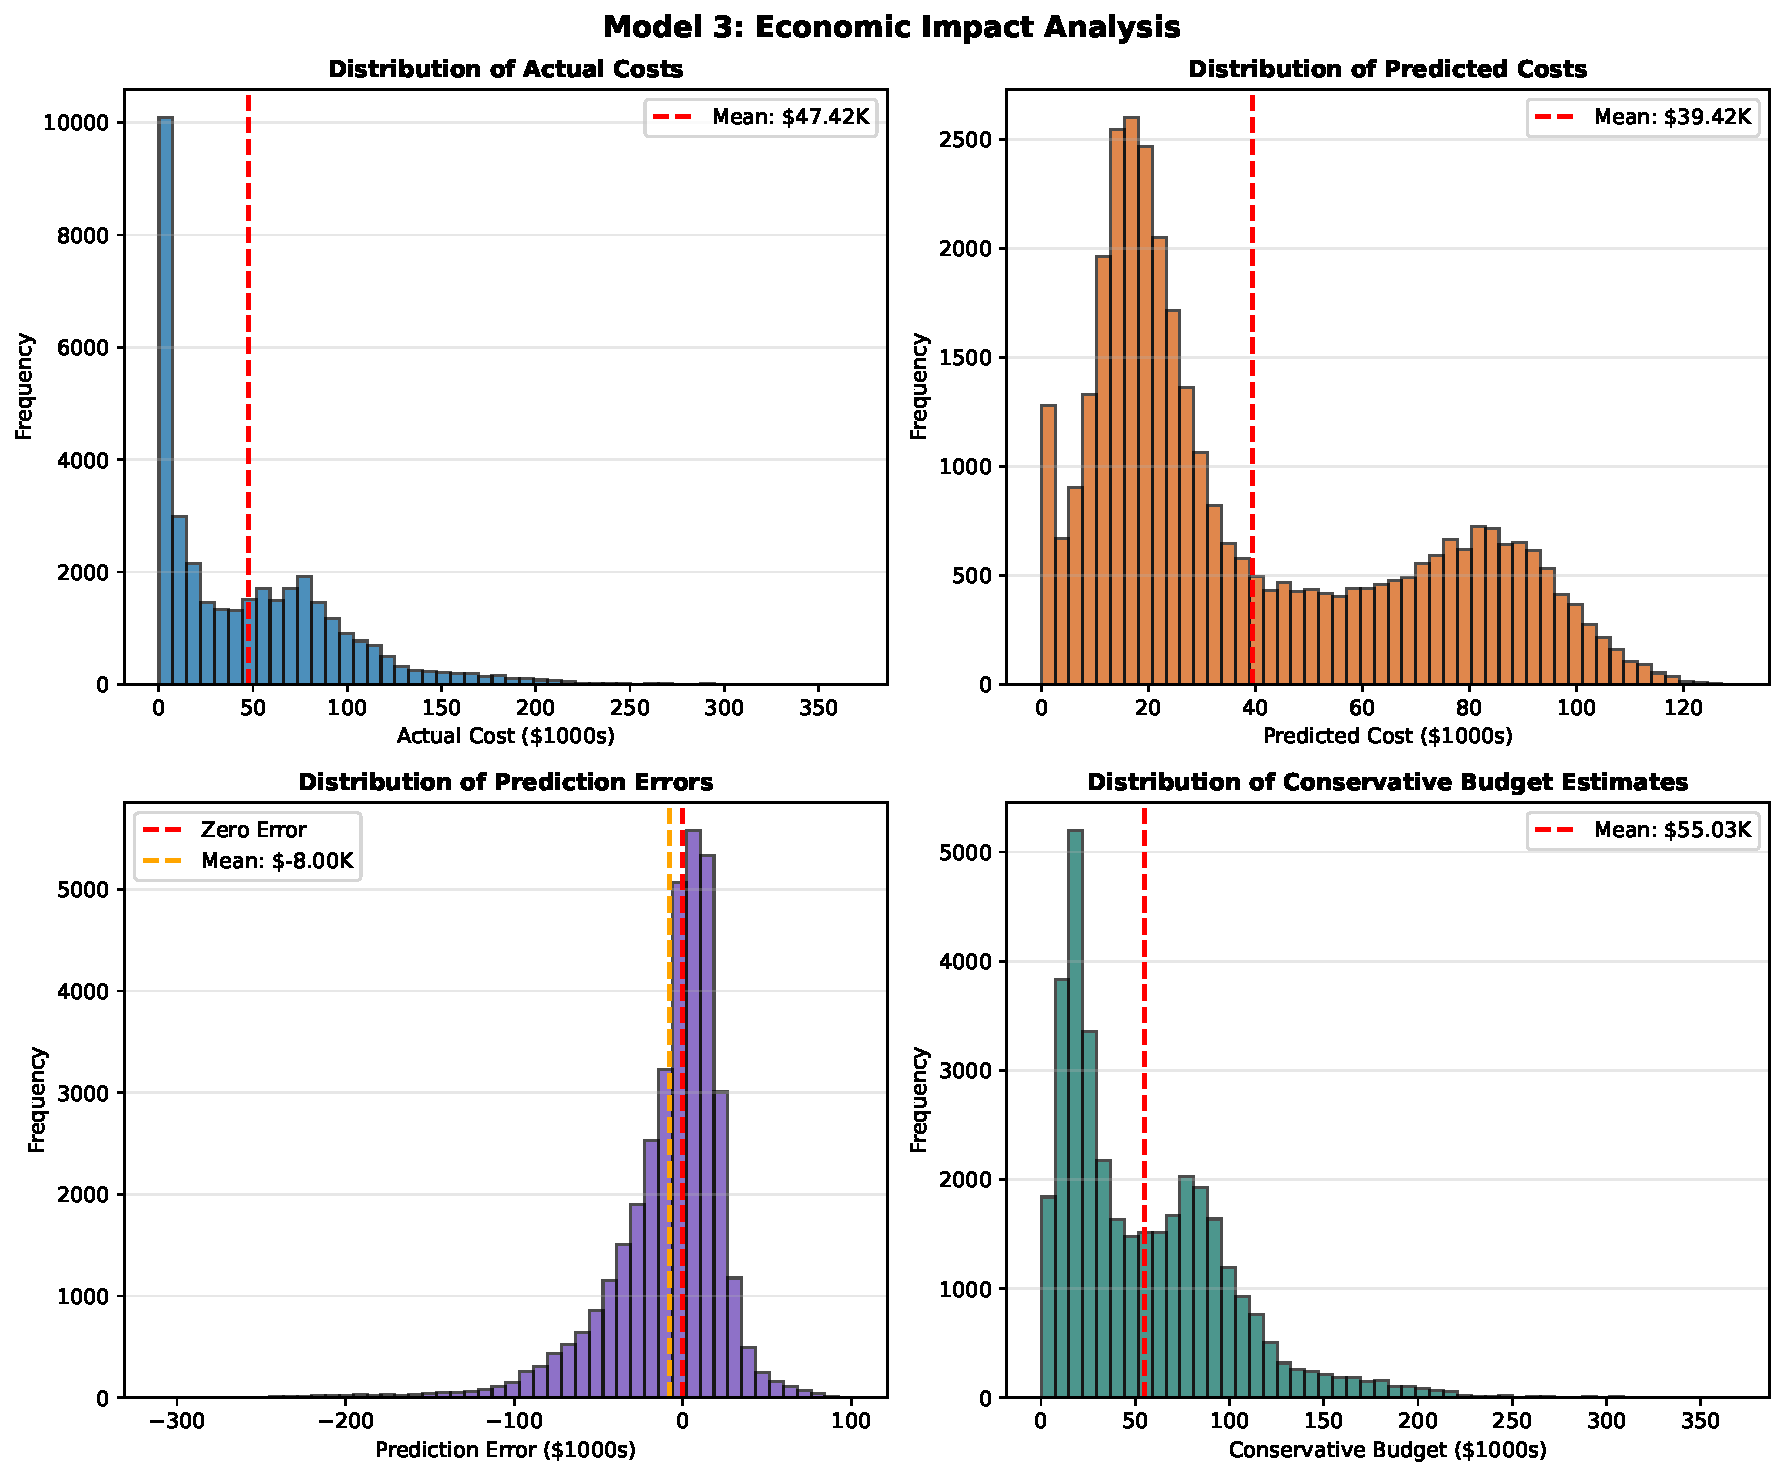
\includegraphics[width=0.95\textwidth]{figures/model_3_Impact_Histograms.pdf}
\caption{Model 3: Distribution of costs, predictions, errors, and conservative budget estimates. The conservative estimate takes the maximum of actual and predicted costs to ensure adequate funding \FiscalYear.}
\label{fig:model3_impact_histograms}
\end{figure}

The conservative budgeting approach for Model 3 would require an additional \$269,705,100.03 (16.05\%) compared to actual costs, averaging \$7,609.33 per client. The model under-predicted costs in 49.6\% of cases, necessitating the conservative approach to avoid budget shortfalls. Notably, 38.7\% of cases (13,705 clients) require large budget increases exceeding 25\%, highlighting the importance of the conservative approach for high-risk cases. 

\clearpage

\subsection{Model 4: Impact Analysis}
\label{subsec:model4_impact}

\begin{table}[htbp]
\centering
\small
\caption{Model 4: Economic Impact Summary \FiscalYear}
\label{tab:model4_impact_summary}
\begin{tabular}{lrr}
\toprule
\textbf{Metric} & \textbf{Value} & \textbf{Per Client} \\
\midrule
Sample Size & 35,444 & --- \\
\midrule
Total Actual Cost & \$1,680,682,853.91 & \$47,417.98 \\
Total Predicted Cost & \$1,565,446,399.80 & \$44,166.75 \\
Total Conservative Budget & \$2,044,389,939.84 & \$57,679.44 \\
\midrule
\textbf{Economic Impact} & \textbf{\$+363,707,085.93} & \textbf{\$+10,261.46} \\
Impact Percentage & 21.64\% & --- \\
\midrule
Cases Over Budget & 19,402 & 54.7\% \\
\midrule
Model $R^2$ (Test) & 0.4746 & --- \\
RMSE (Test) & \$32,372.08 & --- \\
\bottomrule
\end{tabular}
\end{table}

\begin{table}[htbp]
\centering
\small
\caption{Model 4: Economic Impact by Budget Quartile \FiscalYear}
\label{tab:model4_impact_quartile}
\begin{tabular}{lrrrrr}
\toprule
\textbf{Budget Quartile} & \textbf{N} & \textbf{Mean Actual} & \textbf{Mean Conservative} & \textbf{Impact} & \textbf{Impact \%} \\
\midrule
Q1 (Low) & 8,861 & \$1,815.61 & \$24,140.53 & \$+197,821,110.74 & +1,706.56\% \\
Q2 & 8,861 & \$16,963.90 & \$28,151.37 & \$+99,132,237.83 & +104.10\% \\
Q3 & 8,861 & \$57,199.58 & \$63,129.61 & \$+52,546,021.21 & +10.95\% \\
Q4 (High) & 8,861 & \$113,692.83 & \$115,296.23 & \$+14,207,716.14 & +1.88\% \\
\bottomrule
\end{tabular}
\end{table}

\begin{table}[htbp]
\centering
\small
\caption{Model 4: Distribution by Impact Level \FiscalYear}
\label{tab:model4_impact_distribution}
\begin{tabular}{lrrrrr}
\toprule
\textbf{Impact Level} & \textbf{N} & \textbf{\%} & \textbf{Mean Actual} & \textbf{Mean Impact} & \textbf{Impact \%} \\
\midrule
No Change & 16,042 & 45.3\% & \$78,197.96 & \$+0.00 & +0.00\% \\
Small Increase (0-10\%) & 1,981 & 5.6\% & \$62,904.18 & \$+2,977.48 & +4.82\% \\
Moderate Increase (10-25\%) & 2,087 & 5.9\% & \$54,461.61 & \$+9,188.60 & +17.07\% \\
Large Increase (>25\%) & 15,334 & 43.3\% & \$12,257.51 & \$+22,083.74 & +1,050.79\% \\
\bottomrule
\end{tabular}
\end{table}

Tables~\ref{tab:model4_impact_summary} through \ref{tab:model4_impact_distribution} present detailed subgroup analyses, revealing how economic impact varies across age groups, living settings, budget levels, and impact categories. These breakdowns help identify which populations are most affected by prediction errors and where conservative budgeting has the greatest effect.

Figure~\ref{fig:model4_impact_histograms} presents the distribution analysis for Model 4, showing the distributions of actual costs, predicted costs, prediction errors, and conservative budget estimates.

\begin{figure}[htbp]
\centering
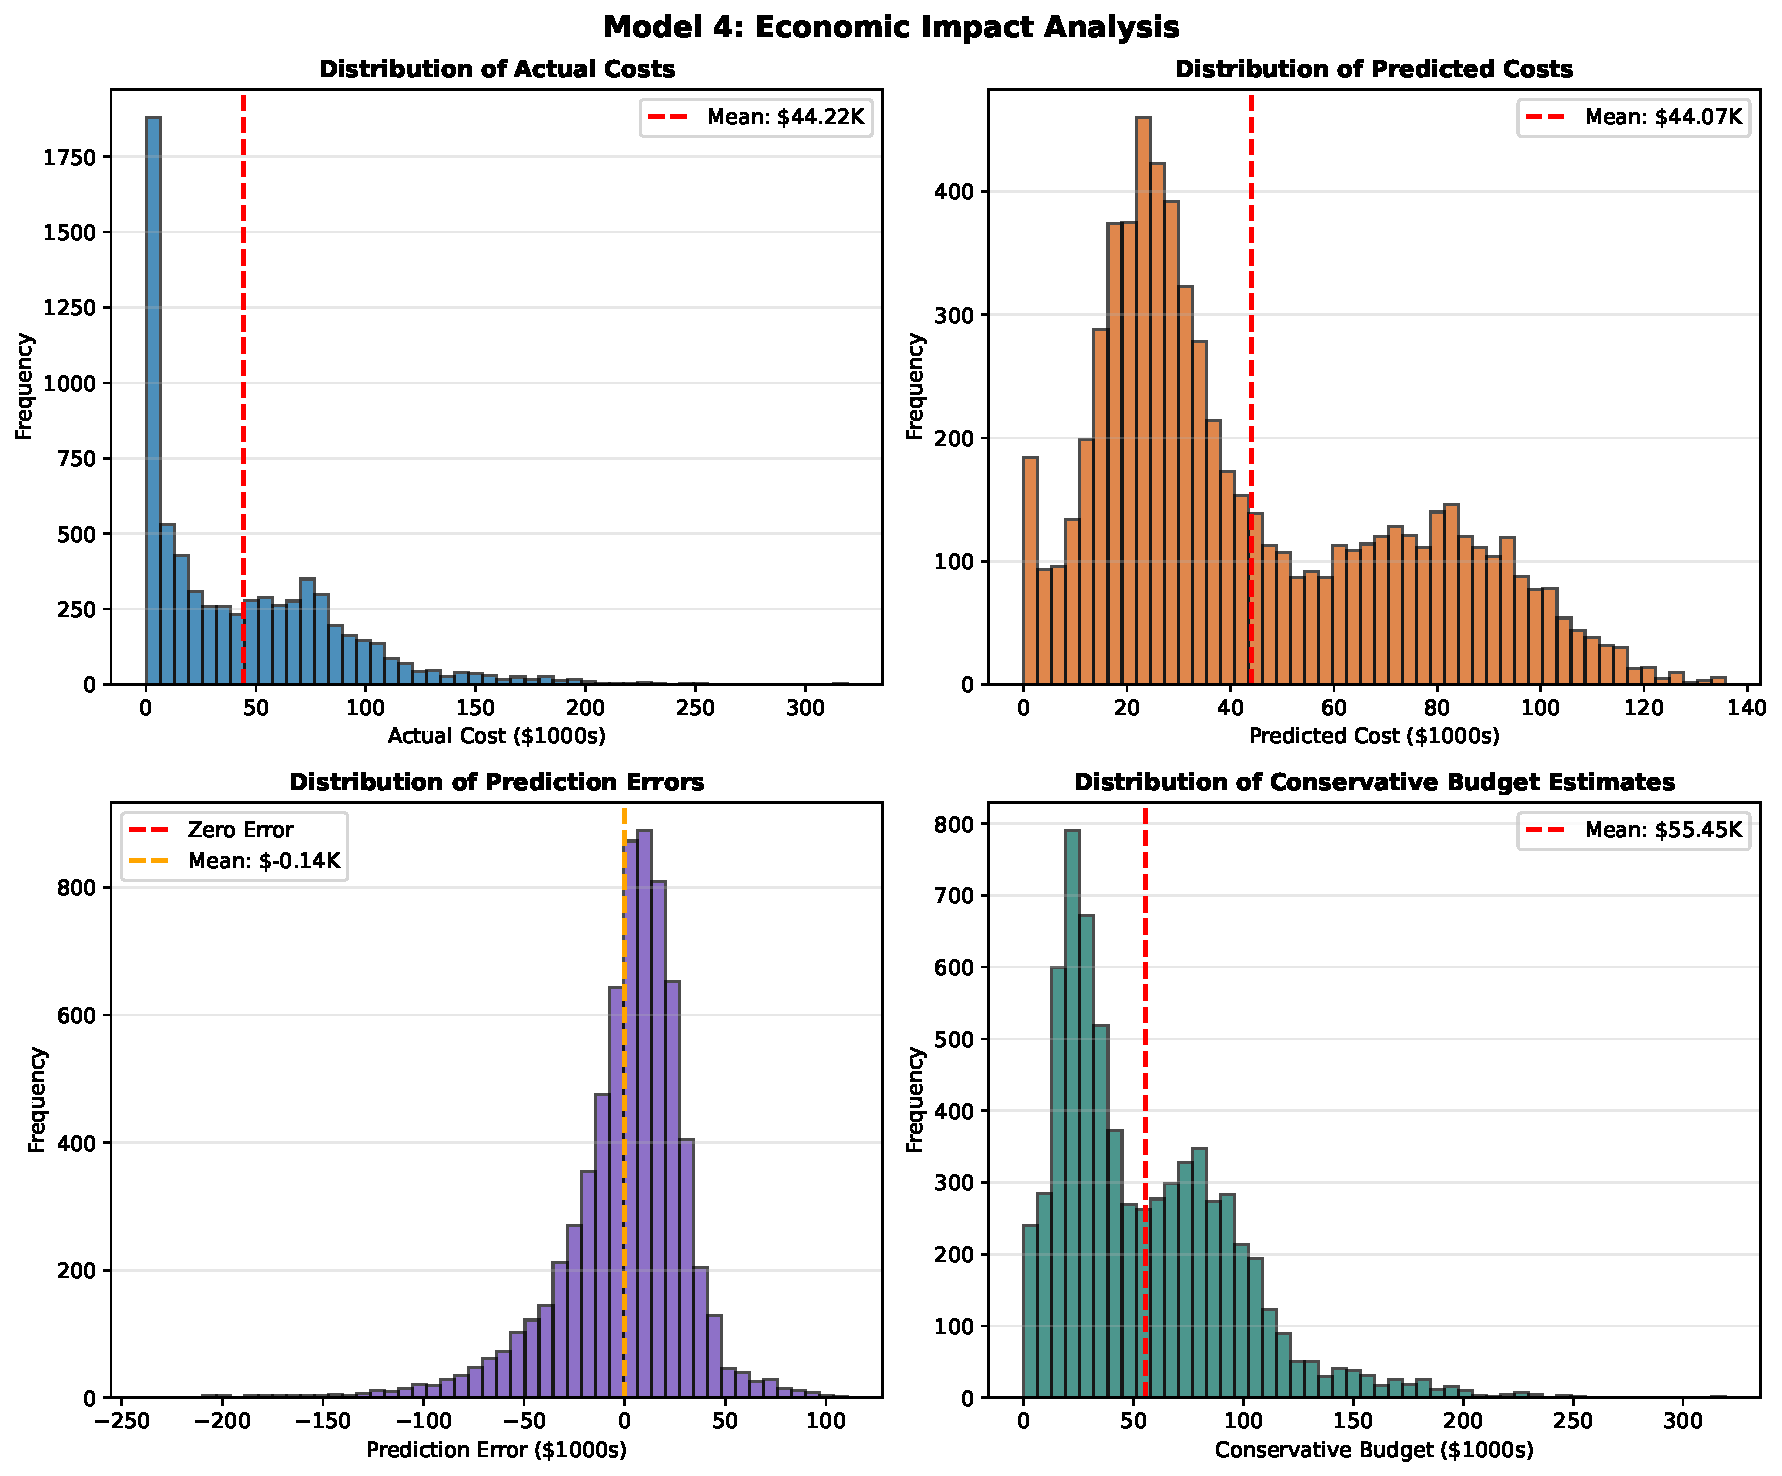
\includegraphics[width=0.95\textwidth]{figures/model_4_Impact_Histograms.pdf}
\caption{Model 4: Distribution of costs, predictions, errors, and conservative budget estimates. The conservative estimate takes the maximum of actual and predicted costs to ensure adequate funding \FiscalYear.}
\label{fig:model4_impact_histograms}
\end{figure}

The conservative budgeting approach for Model 4 would require an additional \$363,707,085.93 (21.64\%) compared to actual costs, averaging \$10,261.46 per client. The model under-predicted costs in 54.7\% of cases, necessitating the conservative approach to avoid budget shortfalls. Notably, 43.3\% of cases (15,334 clients) require large budget increases exceeding 25\%, highlighting the importance of the conservative approach for high-risk cases. 

\clearpage

\subsection{Model 5: Impact Analysis}
\label{subsec:model5_impact}

\begin{table}[htbp]
\centering
\small
\caption{Model 5: Economic Impact Summary \FiscalYear}
\label{tab:model5_impact_summary}
\begin{tabular}{lrr}
\toprule
\textbf{Metric} & \textbf{Value} & \textbf{Per Client} \\
\midrule
Sample Size & 35,444 & --- \\
\midrule
Total Actual Cost & \$1,680,682,853.91 & \$47,417.98 \\
Total Predicted Cost & \$1,573,565,102.29 & \$44,395.81 \\
Total Conservative Budget & \$2,045,365,820.29 & \$57,706.97 \\
\midrule
\textbf{Economic Impact} & \textbf{\$+364,682,966.38} & \textbf{\$+10,288.99} \\
Impact Percentage & 21.70\% & --- \\
\midrule
Cases Over Budget & 19,229 & 54.3\% \\
\midrule
Model $R^2$ (Test) & 0.4772 & --- \\
RMSE (Test) & \$32,290.80 & --- \\
\bottomrule
\end{tabular}
\end{table}

\begin{table}[htbp]
\centering
\small
\caption{Model 5: Economic Impact by Budget Quartile \FiscalYear}
\label{tab:model5_impact_quartile}
\begin{tabular}{lrrrrr}
\toprule
\textbf{Budget Quartile} & \textbf{N} & \textbf{Mean Actual} & \textbf{Mean Conservative} & \textbf{Impact} & \textbf{Impact \%} \\
\midrule
Q1 (Low) & 8,861 & \$1,815.61 & \$23,396.41 & \$+191,227,475.51 & +1,647.56\% \\
Q2 & 8,861 & \$16,963.90 & \$27,870.04 & \$+96,639,318.51 & +100.40\% \\
Q3 & 8,861 & \$57,199.58 & \$63,736.67 & \$+57,925,155.64 & +11.98\% \\
Q4 (High) & 8,861 & \$113,692.83 & \$115,824.76 & \$+18,891,016.72 & +2.48\% \\
\bottomrule
\end{tabular}
\end{table}

\begin{table}[htbp]
\centering
\small
\caption{Model 5: Distribution by Impact Level \FiscalYear}
\label{tab:model5_impact_distribution}
\begin{tabular}{lrrrrr}
\toprule
\textbf{Impact Level} & \textbf{N} & \textbf{\%} & \textbf{Mean Actual} & \textbf{Mean Impact} & \textbf{Impact \%} \\
\midrule
No Change & 16,215 & 45.7\% & \$75,722.29 & \$+0.00 & +0.00\% \\
Small Increase (0-10\%) & 1,969 & 5.6\% & \$65,207.00 & \$+3,175.14 & +4.92\% \\
Moderate Increase (10-25\%) & 2,221 & 6.3\% & \$56,633.60 & \$+9,562.80 & +17.08\% \\
Large Increase (>25\%) & 15,039 & 42.4\% & \$13,210.33 & \$+22,421.18 & +1,035.26\% \\
\bottomrule
\end{tabular}
\end{table}

Tables~\ref{tab:model5_impact_summary} through \ref{tab:model5_impact_distribution} present detailed subgroup analyses, revealing how economic impact varies across age groups, living settings, budget levels, and impact categories. These breakdowns help identify which populations are most affected by prediction errors and where conservative budgeting has the greatest effect.

Figure~\ref{fig:model5_impact_histograms} presents the distribution analysis for Model 5, showing the distributions of actual costs, predicted costs, prediction errors, and conservative budget estimates.

\begin{figure}[htbp]
\centering
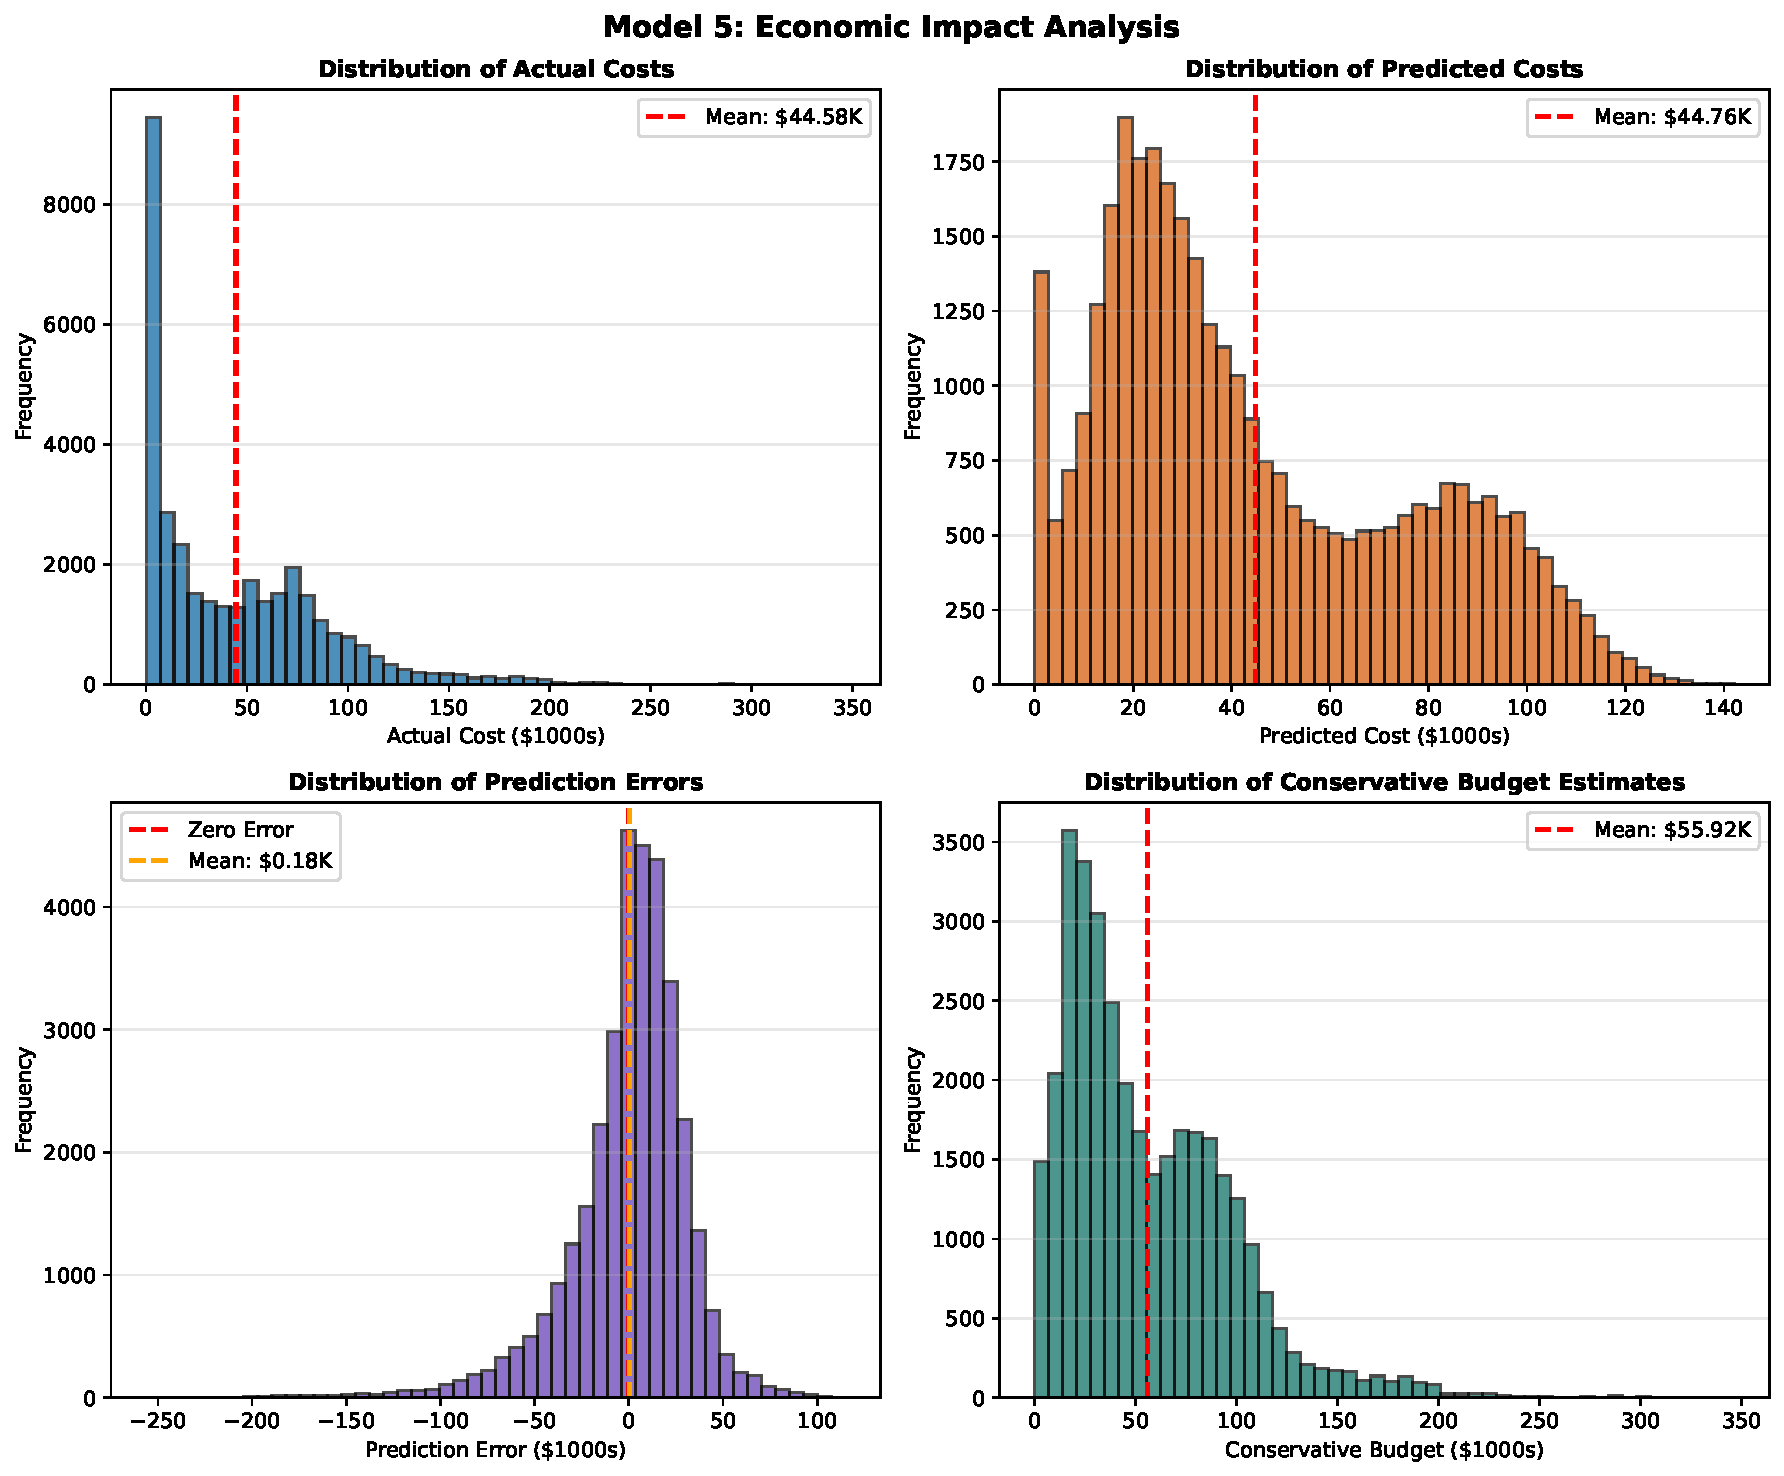
\includegraphics[width=0.95\textwidth]{figures/model_5_Impact_Histograms.pdf}
\caption{Model 5: Distribution of costs, predictions, errors, and conservative budget estimates. The conservative estimate takes the maximum of actual and predicted costs to ensure adequate funding \FiscalYear.}
\label{fig:model5_impact_histograms}
\end{figure}

The conservative budgeting approach for Model 5 would require an additional \$364,682,966.38 (21.70\%) compared to actual costs, averaging \$10,288.99 per client. The model under-predicted costs in 54.3\% of cases, necessitating the conservative approach to avoid budget shortfalls. Notably, 42.4\% of cases (15,039 clients) require large budget increases exceeding 25\%, highlighting the importance of the conservative approach for high-risk cases. 

\clearpage

\subsection{Model 6: Impact Analysis}
\label{subsec:model6_impact}

\begin{table}[htbp]
\centering
\small
\caption{Model 6: Economic Impact Summary \FiscalYear}
\label{tab:model6_impact_summary}
\begin{tabular}{lrr}
\toprule
\textbf{Metric} & \textbf{Value} & \textbf{Per Client} \\
\midrule
Sample Size & 35,444 & --- \\
\midrule
Total Actual Cost & \$1,680,682,853.91 & \$47,417.98 \\
Total Predicted Cost & \$2,168,063,052.31 & \$61,168.69 \\
Total Conservative Budget & \$2,551,176,818.24 & \$71,977.68 \\
\midrule
\textbf{Economic Impact} & \textbf{\$+870,493,964.33} & \textbf{\$+24,559.70} \\
Impact Percentage & 51.79\% & --- \\
\midrule
Cases Over Budget & 24,153 & 68.1\% \\
\midrule
Model $R^2$ (Test) & -0.3517 & --- \\
RMSE (Test) & \$51,923.33 & --- \\
\bottomrule
\end{tabular}
\end{table}

\begin{table}[htbp]
\centering
\small
\caption{Model 6: Economic Impact by Budget Quartile \FiscalYear}
\label{tab:model6_impact_quartile}
\begin{tabular}{lrrrrr}
\toprule
\textbf{Budget Quartile} & \textbf{N} & \textbf{Mean Actual} & \textbf{Mean Conservative} & \textbf{Impact} & \textbf{Impact \%} \\
\midrule
Q1 (Low) & 8,861 & \$1,815.61 & \$19,022.50 & \$+152,470,243.96 & +1,326.71\% \\
Q2 & 8,861 & \$16,963.90 & \$28,400.50 & \$+101,339,752.86 & +96.51\% \\
Q3 & 8,861 & \$57,199.58 & \$86,599.32 & \$+260,511,116.53 & +49.82\% \\
Q4 (High) & 8,861 & \$113,692.83 & \$153,888.39 & \$+356,172,850.99 & +40.77\% \\
\bottomrule
\end{tabular}
\end{table}

\begin{table}[htbp]
\centering
\small
\caption{Model 6: Distribution by Impact Level \FiscalYear}
\label{tab:model6_impact_distribution}
\begin{tabular}{lrrrrr}
\toprule
\textbf{Impact Level} & \textbf{N} & \textbf{\%} & \textbf{Mean Actual} & \textbf{Mean Impact} & \textbf{Impact \%} \\
\midrule
No Change & 11,291 & 31.9\% & \$68,665.60 & \$+0.00 & +0.00\% \\
Small Increase (0-10\%) & 1,123 & 3.2\% & \$61,881.32 & \$+3,189.49 & +5.03\% \\
Moderate Increase (10-25\%) & 1,539 & 4.3\% & \$64,883.40 & \$+11,269.98 & +17.41\% \\
Large Increase (>25\%) & 21,491 & 60.6\% & \$34,248.35 & \$+39,531.32 & +622.65\% \\
\bottomrule
\end{tabular}
\end{table}

Tables~\ref{tab:model6_impact_summary} through \ref{tab:model6_impact_distribution} present detailed subgroup analyses, revealing how economic impact varies across age groups, living settings, budget levels, and impact categories. These breakdowns help identify which populations are most affected by prediction errors and where conservative budgeting has the greatest effect.

Figure~\ref{fig:model6_impact_histograms} presents the distribution analysis for Model 6, showing the distributions of actual costs, predicted costs, prediction errors, and conservative budget estimates.

\begin{figure}[htbp]
\centering
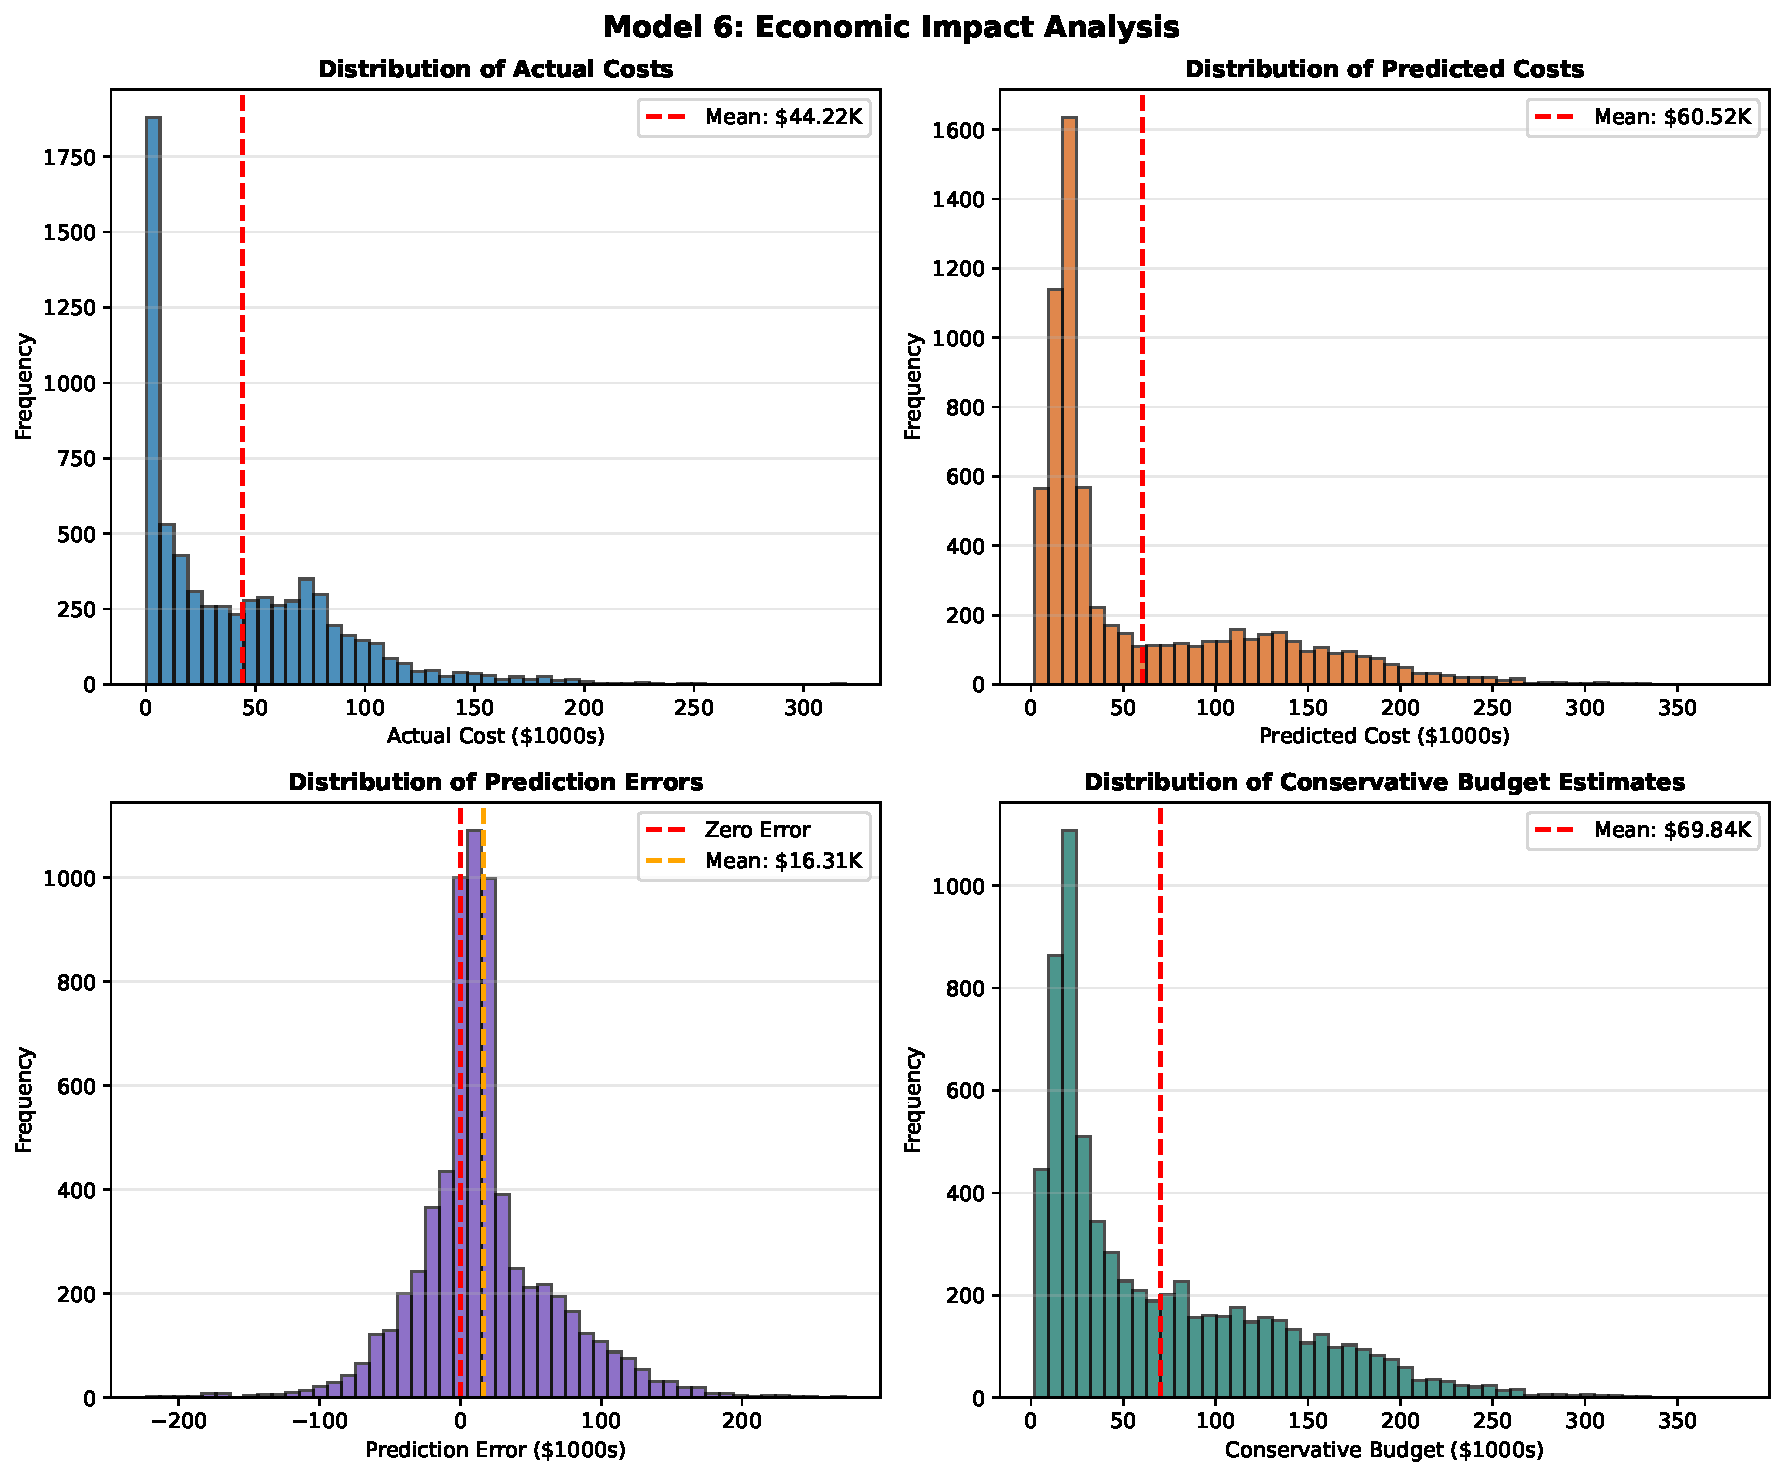
\includegraphics[width=0.95\textwidth]{figures/model_6_Impact_Histograms.pdf}
\caption{Model 6: Distribution of costs, predictions, errors, and conservative budget estimates. The conservative estimate takes the maximum of actual and predicted costs to ensure adequate funding \FiscalYear.}
\label{fig:model6_impact_histograms}
\end{figure}

The conservative budgeting approach for Model 6 would require an additional \$870,493,964.33 (51.79\%) compared to actual costs, averaging \$24,559.70 per client. The model under-predicted costs in 68.1\% of cases, necessitating the conservative approach to avoid budget shortfalls. Notably, 60.6\% of cases (21,491 clients) require large budget increases exceeding 25\%, highlighting the importance of the conservative approach for high-risk cases. 

\clearpage

\subsection{Model 9: Impact Analysis}
\label{subsec:model9_impact}

\begin{table}[htbp]
\centering
\small
\caption{Model 9: Economic Impact Summary \FiscalYear}
\label{tab:model9_impact_summary}
\begin{tabular}{lrr}
\toprule
\textbf{Metric} & \textbf{Value} & \textbf{Per Client} \\
\midrule
Sample Size & 35,444 & --- \\
\midrule
Total Actual Cost & \$1,680,682,853.91 & \$47,417.98 \\
Total Predicted Cost & \$1,413,102,733.23 & \$39,868.60 \\
Total Conservative Budget & \$1,902,497,860.41 & \$53,676.16 \\
\midrule
\textbf{Economic Impact} & \textbf{\$+221,815,006.50} & \textbf{\$+6,258.18} \\
Impact Percentage & 13.20\% & --- \\
\midrule
Cases Over Budget & 16,750 & 47.3\% \\
\midrule
Model $R^2$ (Test) & 0.6412 & --- \\
RMSE (Test) & \$24,727.15 & --- \\
\bottomrule
\end{tabular}
\end{table}

\begin{table}[htbp]
\centering
\small
\caption{Model 9: Economic Impact by Budget Quartile \FiscalYear}
\label{tab:model9_impact_quartile}
\begin{tabular}{lrrrrr}
\toprule
\textbf{Budget Quartile} & \textbf{N} & \textbf{Mean Actual} & \textbf{Mean Conservative} & \textbf{Impact} & \textbf{Impact \%} \\
\midrule
Q1 (Low) & 8,861 & \$1,815.61 & \$17,710.57 & \$+140,845,254.66 & +1,281.94\% \\
Q2 & 8,861 & \$16,963.90 & \$23,290.13 & \$+56,056,721.85 & +64.17\% \\
Q3 & 8,861 & \$57,199.58 & \$59,449.32 & \$+19,934,949.20 & +4.31\% \\
Q4 (High) & 8,861 & \$113,692.83 & \$114,254.63 & \$+4,978,080.79 & +0.65\% \\
\bottomrule
\end{tabular}
\end{table}

\begin{table}[htbp]
\centering
\small
\caption{Model 9: Distribution by Impact Level \FiscalYear}
\label{tab:model9_impact_distribution}
\begin{tabular}{lrrrrr}
\toprule
\textbf{Impact Level} & \textbf{N} & \textbf{\%} & \textbf{Mean Actual} & \textbf{Mean Impact} & \textbf{Impact \%} \\
\midrule
No Change & 18,694 & 52.7\% & \$76,659.94 & \$+0.00 & +0.00\% \\
Small Increase (0-10\%) & 1,760 & 5.0\% & \$52,090.90 & \$+2,373.54 & +4.69\% \\
Moderate Increase (10-25\%) & 1,546 & 4.4\% & \$39,548.57 & \$+6,561.35 & +16.94\% \\
Large Increase (>25\%) & 13,444 & 37.9\% & \$7,049.97 & \$+15,433.93 & +887.93\% \\
\bottomrule
\end{tabular}
\end{table}

Tables~\ref{tab:model9_impact_summary} through \ref{tab:model9_impact_distribution} present detailed subgroup analyses, revealing how economic impact varies across age groups, living settings, budget levels, and impact categories. These breakdowns help identify which populations are most affected by prediction errors and where conservative budgeting has the greatest effect.

Figure~\ref{fig:model9_impact_histograms} presents the distribution analysis for Model 9, showing the distributions of actual costs, predicted costs, prediction errors, and conservative budget estimates.

\begin{figure}[htbp]
\centering
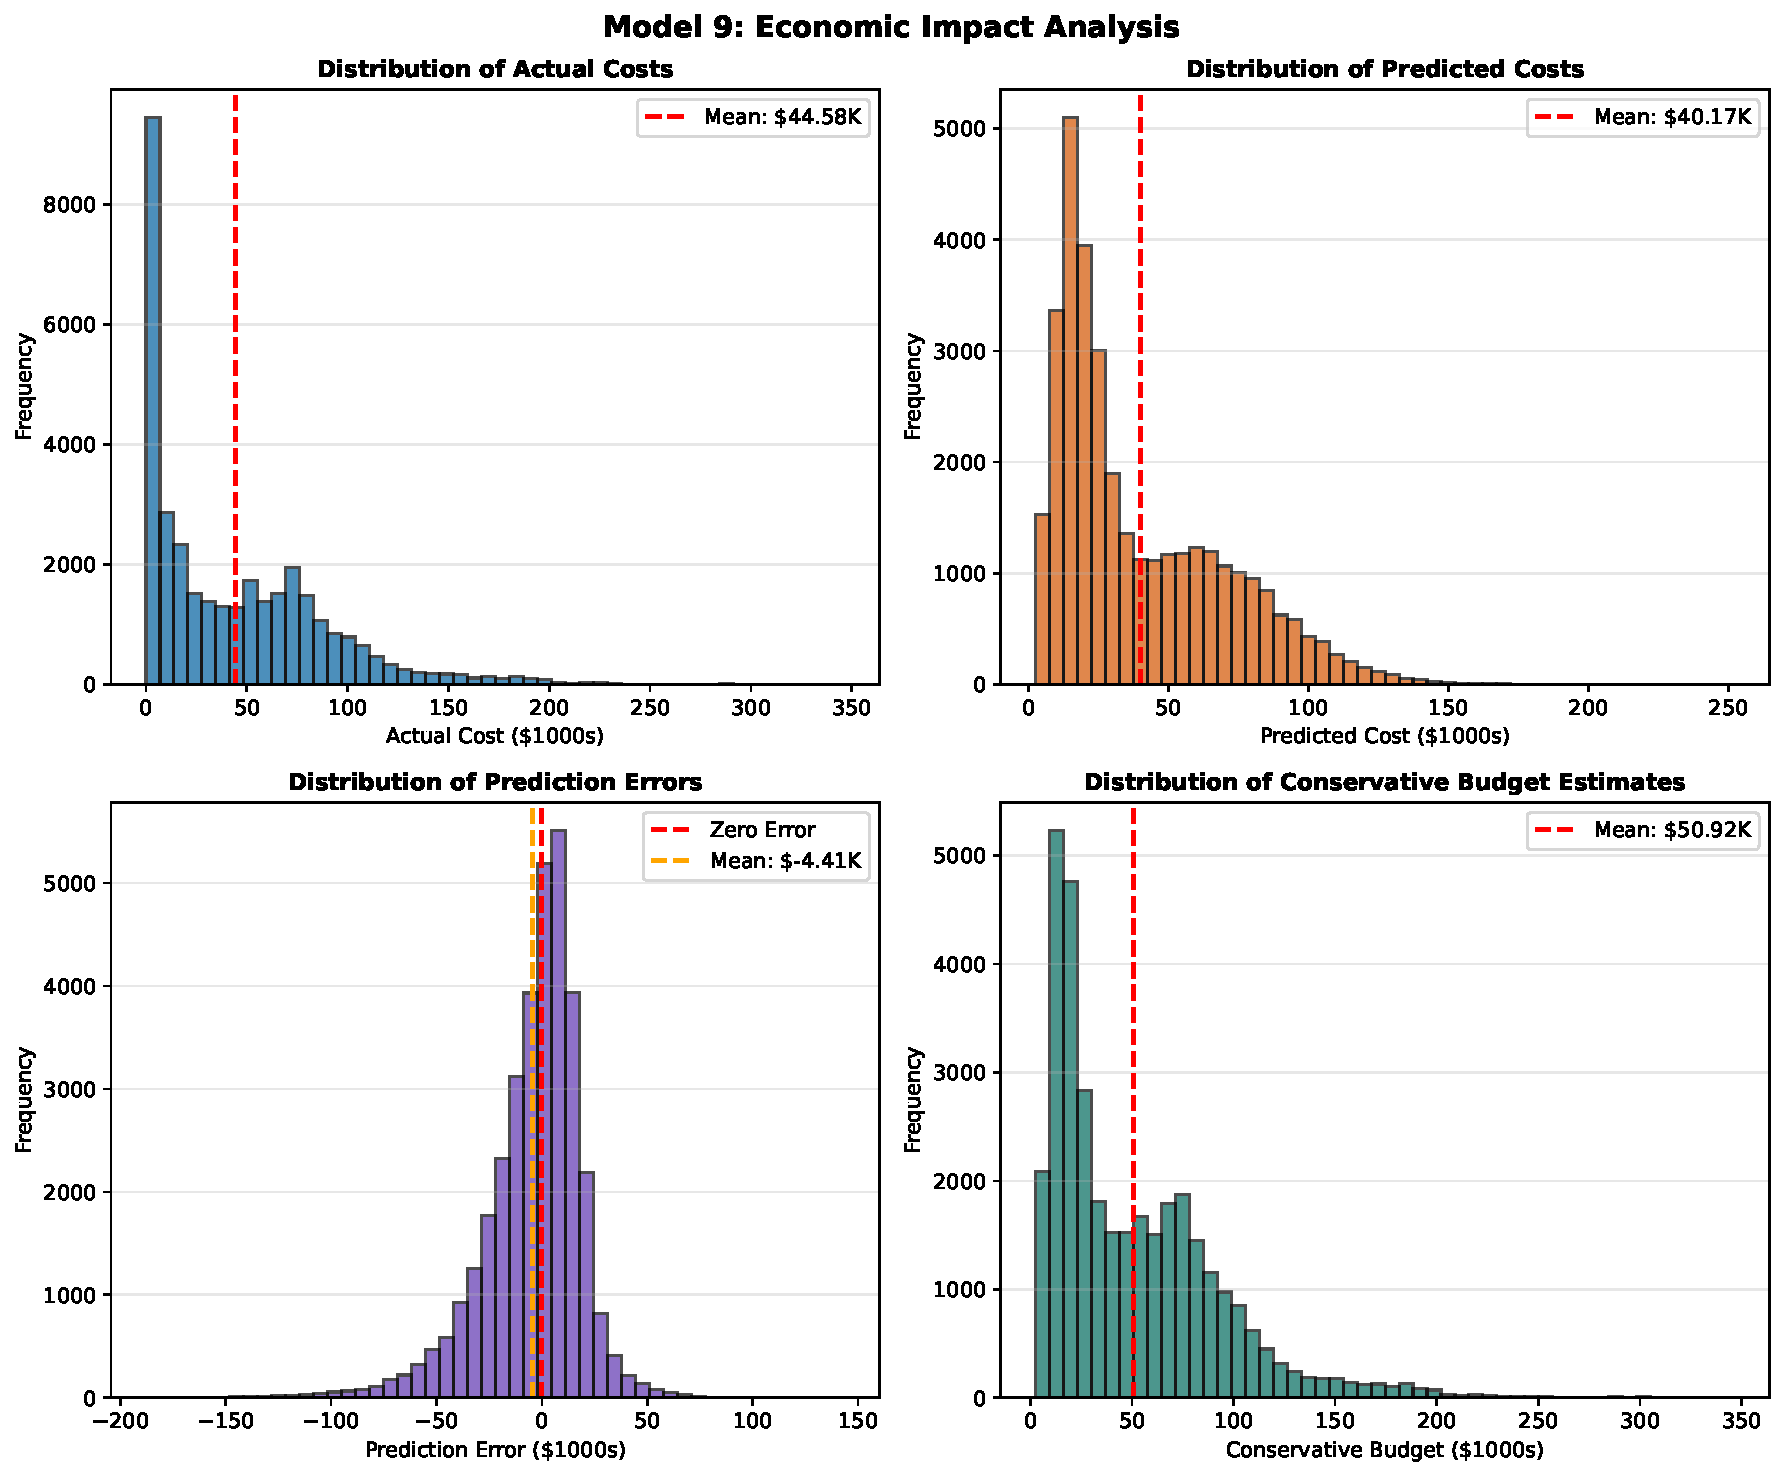
\includegraphics[width=0.95\textwidth]{figures/model_9_Impact_Histograms.pdf}
\caption{Model 9: Distribution of costs, predictions, errors, and conservative budget estimates. The conservative estimate takes the maximum of actual and predicted costs to ensure adequate funding \FiscalYear.}
\label{fig:model9_impact_histograms}
\end{figure}

The conservative budgeting approach for Model 9 would require an additional \$221,815,006.50 (13.20\%) compared to actual costs, averaging \$6,258.18 per client. The model under-predicted costs in 47.3\% of cases, necessitating the conservative approach to avoid budget shortfalls. Notably, 37.9\% of cases (13,444 clients) require large budget increases exceeding 25\%, highlighting the importance of the conservative approach for high-risk cases. 

\clearpage

\section{Comparative Analysis Across Models }
\label{subsec:comparative_impact}

Table~\ref{tab:all_models_impact_comparison} presents a comprehensive comparison of economic impacts across all budget allocation models.

\begin{table}[htbp]
\centering
\small
\caption{Comparative Economic Impact Analysis Across All Models \FiscalYear}
\label{tab:all_models_impact_comparison}
\begin{tabular}{lrrrrr}
\toprule
\textbf{Model} & \textbf{Samples} & \textbf{$R^2$ Test} & \textbf{Economic Impact} & \textbf{Impact \%} & \textbf{Over Budget \%} \\
\midrule
Model 1 & 35,444 & 0.4300 & \$+228,192,164.33 & +13.58\% & 48.5\% \\
Model 2 & 35,444 & 0.4386 & \$+397,973,790.19 & +23.68\% & 58.6\% \\
Model 3 & 35,444 & 0.4534 & \$+269,705,100.03 & +16.05\% & 49.6\% \\
Model 4 & 35,444 & 0.4746 & \$+363,707,085.93 & +21.64\% & 54.7\% \\
Model 5 & 35,444 & 0.4772 & \$+364,682,966.38 & +21.70\% & 54.3\% \\
Model 6 & 35,444 & -0.3517 & \$+870,493,964.33 & +51.79\% & 68.1\% \\
Model 9 & 35,444 & 0.6412 & \$+221,815,006.50 & +13.20\% & 47.3\% \\
\bottomrule
\end{tabular}
\end{table}

\section{Key Insights}

\begin{itemize}
\item Model 9 achieves the highest predictive accuracy with $R^2$ = 0.6412.
\item Model 6 requires the largest conservative budget adjustment at 51.79\%.
\item The conservative budgeting approach ensures adequate funding to cover cases where the model under-predicts actual costs.
\item Economic impact percentages reflect both model accuracy and the degree of systematic under- or over-prediction.
\item Subgroup analyses reveal differential impacts across age groups, living settings, and budget levels, providing insights for targeted policy interventions.
\item Impact level distributions identify high-risk cases requiring substantial budget adjustments beyond model predictions.
\end{itemize}

